\section{Schedule and Budget}

The proposed schedule and estimate of costs for the 35t prototype RCE-based DAQ is shown in Fig. \ref{fig:budget35t}.  

\begin{figure}[htb]
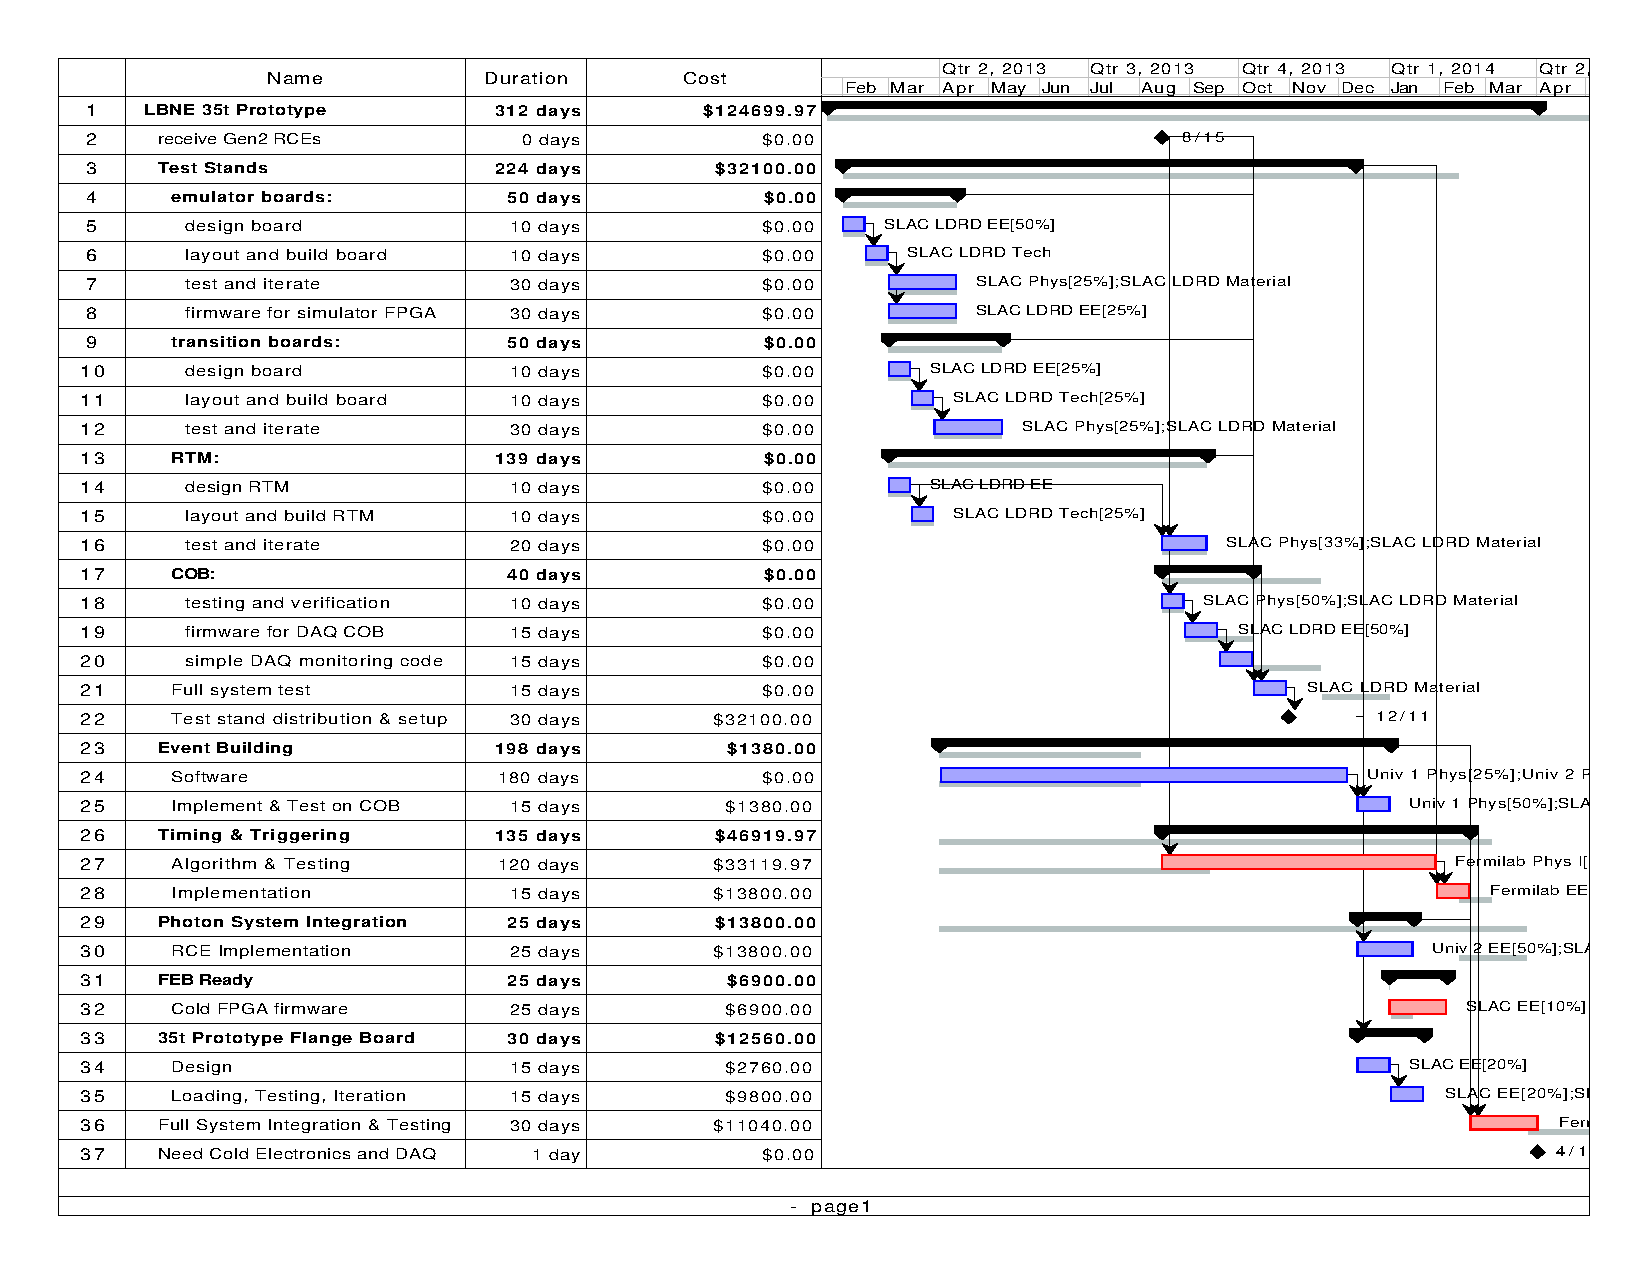
\includegraphics[scale=0.8,angle=90]{project-gantt.pdf}
\caption{Schedule and budget for the 35t RCE-based DAQ.}
\label{fig:budget35t}
\end{figure} 

This proposal uses the Gen-3 COBs which are expected to be available in September   at the latest.  The Gen-3 COBs will use the Virtex ZYNQ SoC (series-7) which has many advantages over the series-5 previously used.  Probably the most important feature for our purposes is that it is distributed with with a Linux distribution.  This makes software development much simpler; we can develop our algorithms in C++ on a Linux PC and simply copy them directly to the RCEs.  

The budget includes 4 DAQ test stands composed of a 2-slot ATCA crate (with power), a COB and RTM, a mezzanine board with a single RCE, a simplified flange board, and an emulation board.  The emulation board will consist of a Virtex-5 FPGA programmed to output data with format and rate  similar to that expected from the TPC FEB and transmit it to the flange board via copper.  The test stands will allow us to develop the DAQ system at places other than at SLAC.  One of these test stands can likely be used for the 35t DAQ system.    Much of the development needed to get the first test-stand working will be covered under a SLAC LDRD so, for project purposes, is considered to be available at no cost.  

There are a number of tasks necessary for the complete working system that can be done semi-independently of the full ATCA-based DAQ.  Preliminary work on some of these items can start immediately on test boards or PCs which is advantageous because we don't expect to receive the Gen-3 boards until August.  All of the tasks listed can be performed by non-SLAC labs or universities with a low-level of SLAC support.  
\begin{itemize}
\item \textbf{Timing/Trigger:  }The external clock (and possibly trigger) must be integrated into the RTM/COB and distributed to the FEBs.  Much of this work likely requires a COB.  Details on the clock and trigger signals may be necessary for RTM design.   The existing NOvA timing units may be a good match for the 35t prototype; in this case the output of that system must be integrated the RCE-based design.  
\item \textbf{Event Building:  }If desired, some level of event building can be performed in the COBs before sending to the PC farm.  This work can be done by a physicist and can be started at any time with C++ code on a Linux PC and be transfered to the RCEs when ready.   
\item \textbf{PGP \& Other Firmware on FEB:   } Once the FEB is laid out,  we can used a PCIe-based PGP card to program  the cold FPGA (up to timing/trigger, which will require the COB).  This task requires an EE but the procedure is well documented.  The firmware for the clock must also be written as well as the control interface between the FPGA and the RCEs.  
% \item \textbf{Photon Detector (PD):  }The PD for the 35t will be read out using a CAEN DT5740 32-channel digitizer.  The output of the digitizer is either USB or fiber optic (with CAEN propriety protocol).   Depending on where the PD signals are combined with the TPC data stream, a new RTM design may be needed and some, small amount of firmware written.  However, if the PD stream is combined on the farm nodes, then the RCE-based design is unaffected (apart from possibly integrating the timing).  The design of this can be done independently of the COB.  
\item \textbf{Run Control:  }  The interface between the ATCA crate, COBs, FEBs, etc and run control must be developed. Many tools exist for controlling the RCEs and the crate, but they must be integrated into run control.  This likely requires a test stand to do but much of the work can be done by a physicist.  
\end{itemize}


%================
\begin{table}[tbh]
\begin{center}
\begin{tabular}{|l|c|c|}   
\hline \hline 
    & Hours  & Cost (\$1k) \\      
\hline
   Physicist           & 1350 &0 \\ 
   Engineer           & 503   &58 \\ 
   Technician        & 32    &3\\ 
\hline \hline
\end{tabular}
\caption[]{Total number of work hours and assumed cost for the 35t Prototype.}
\label{tab:labor} 
\end{center}
\end{table}
%=================





%================
\begin{table}[tbh]
\begin{center}
\begin{tabular}{|l|c|cc|cc|}   
\hline \hline 
						 			 &         & \multicolumn{2}{|c|}{35t  Prototype + Test Stands} &\multicolumn{2}{|c|}{Full LBNE }    \\      
									 & Unit Cost (\$)& Count &  Total Cost (\$) & Count &  Total Cost  (\$)\\      
\hline
   2-Slot ATCA Shelf    & 3,500              &  3         &    10,500     &  ---  &  ---  \\ 
  14-Slot ATCA Shelf   & 6,500              &  ---         &    ---    &  4  &  26,000  \\ 
     RTM+COBs             & 3,500              &  3         &    10,500     &    50   &   175,000\\ 
   Mezanine Board     & 350                &  5         &       1,050    &  16   &  5,600 \\ 
   Zynq-based RCE	   & 650                &  8          &   5,200        &   32    &208,000\\ 
   Flange Boards          & 1,500              &  4          &  6000        & 50          & 75,000\\ 
   Emulation Boards     & 1,500              &  4          &  6000        &  ---        &    ---  \\ 
\hline \hline
\end{tabular}
\caption[]{Estimated materials cost of the back-end DAQ for 35t and the full 10kt LBNE.}
\label{tab:mats} 
\end{center}
\end{table}
%=================

